% Options for packages loaded elsewhere
\PassOptionsToPackage{unicode}{hyperref}
\PassOptionsToPackage{hyphens}{url}
%
\documentclass[
  12pt,
]{article}
\usepackage{amsmath,amssymb}
\usepackage{lmodern}
\usepackage{iftex}
\ifPDFTeX
  \usepackage[T1]{fontenc}
  \usepackage[utf8]{inputenc}
  \usepackage{textcomp} % provide euro and other symbols
\else % if luatex or xetex
  \usepackage{unicode-math}
  \defaultfontfeatures{Scale=MatchLowercase}
  \defaultfontfeatures[\rmfamily]{Ligatures=TeX,Scale=1}
\fi
% Use upquote if available, for straight quotes in verbatim environments
\IfFileExists{upquote.sty}{\usepackage{upquote}}{}
\IfFileExists{microtype.sty}{% use microtype if available
  \usepackage[]{microtype}
  \UseMicrotypeSet[protrusion]{basicmath} % disable protrusion for tt fonts
}{}
\makeatletter
\@ifundefined{KOMAClassName}{% if non-KOMA class
  \IfFileExists{parskip.sty}{%
    \usepackage{parskip}
  }{% else
    \setlength{\parindent}{0pt}
    \setlength{\parskip}{6pt plus 2pt minus 1pt}}
}{% if KOMA class
  \KOMAoptions{parskip=half}}
\makeatother
\usepackage{xcolor}
\IfFileExists{xurl.sty}{\usepackage{xurl}}{} % add URL line breaks if available
\IfFileExists{bookmark.sty}{\usepackage{bookmark}}{\usepackage{hyperref}}
\hypersetup{
  pdftitle={Temporal variation in the prokaryotic community of a nearshore marine environment},
  hidelinks,
  pdfcreator={LaTeX via pandoc}}
\urlstyle{same} % disable monospaced font for URLs
\usepackage[margin = 1.0in]{geometry}
\usepackage{graphicx}
\makeatletter
\def\maxwidth{\ifdim\Gin@nat@width>\linewidth\linewidth\else\Gin@nat@width\fi}
\def\maxheight{\ifdim\Gin@nat@height>\textheight\textheight\else\Gin@nat@height\fi}
\makeatother
% Scale images if necessary, so that they will not overflow the page
% margins by default, and it is still possible to overwrite the defaults
% using explicit options in \includegraphics[width, height, ...]{}
\setkeys{Gin}{width=\maxwidth,height=\maxheight,keepaspectratio}
% Set default figure placement to htbp
\makeatletter
\def\fps@figure{htbp}
\makeatother
\setlength{\emergencystretch}{3em} % prevent overfull lines
\providecommand{\tightlist}{%
  \setlength{\itemsep}{0pt}\setlength{\parskip}{0pt}}
\setcounter{secnumdepth}{-\maxdimen} % remove section numbering
\newlength{\cslhangindent}
\setlength{\cslhangindent}{1.5em}
\newlength{\csllabelwidth}
\setlength{\csllabelwidth}{3em}
\newlength{\cslentryspacingunit} % times entry-spacing
\setlength{\cslentryspacingunit}{\parskip}
\newenvironment{CSLReferences}[2] % #1 hanging-ident, #2 entry spacing
 {% don't indent paragraphs
  \setlength{\parindent}{0pt}
  % turn on hanging indent if param 1 is 1
  \ifodd #1
  \let\oldpar\par
  \def\par{\hangindent=\cslhangindent\oldpar}
  \fi
  % set entry spacing
  \setlength{\parskip}{#2\cslentryspacingunit}
 }%
 {}
\usepackage{calc}
\newcommand{\CSLBlock}[1]{#1\hfill\break}
\newcommand{\CSLLeftMargin}[1]{\parbox[t]{\csllabelwidth}{#1}}
\newcommand{\CSLRightInline}[1]{\parbox[t]{\linewidth - \csllabelwidth}{#1}\break}
\newcommand{\CSLIndent}[1]{\hspace{\cslhangindent}#1}
\usepackage{times}
\usepackage[T1]{fontenc}

\usepackage[none]{hyphenat}

\usepackage{setspace}
\doublespacing
\setlength{\parskip}{1em}

\usepackage{lineno}
\renewcommand{\linenumberfont}{\normalfont\tiny}

\usepackage{pdfpages}

\usepackage{indentfirst}

\usepackage[labelsep=period, labelfont=bf]{caption}
\renewcommand{\thefigure}{\arabic{figure}}
\renewcommand{\figurename}{Figure}

\usepackage{pdflscape}
\newcommand{\blandscape}{\begin{landscape}}
\newcommand{\elandscape}{\end{landscape}}

\usepackage{siunitx}
\DeclareSIUnit\molar{\mole\per\cubic\deci\metre}
\DeclareSIUnit\Molar{\textsc{m}}
\DeclareSIUnit\cells{\text{cells}}
\DeclareSIUnit\litre{l}

\usepackage{caption}
\captionsetup{justification=justified}

\usepackage{float}

\usepackage{xr}
\externaldocument[supp-]{supplementary}

\usepackage{txfonts}

\renewcommand{\figureautorefname}{Fig.}

\usepackage{microtype}

\usepackage{chemformula}
\ifLuaTeX
  \usepackage{selnolig}  % disable illegal ligatures
\fi

\title{\textbf{Temporal variation in the prokaryotic community of a
nearshore marine environment}}
\author{}
\date{\vspace{-2.5em}}

\begin{document}
\maketitle

\vspace{20mm}

Marino Korlević\textsuperscript{1*}, Marsej
Markovski\textsuperscript{1}, Gerhard J. Herndl\textsuperscript{2,3},
and Mirjana Najdek\textsuperscript{1}

1. Center for Marine Research, Ruđer Bošković Institute, Croatia

2. Department of Functional and Evolutionary Ecology, University of
Vienna, Austria

3. Department of Marine Microbiology and Biogeochemistry, Royal
Netherlands Institute for Sea Research (NIOZ), Utrecht University, The
Netherlands

\textsuperscript{*}To whom correspondence should be addressed:

Marino Korlević

G. Paliaga 5, 52210 Rovinj, Croatia

Tel.: +385 52 804 768

Fax: +385 52 804 780

e-mail:
\href{mailto:marino.korlevic@irb.hr}{\nolinkurl{marino.korlevic@irb.hr}}

\newpage
\linenumbers
\sisetup{mode = text}
\setlength\parindent{24pt}

\hypertarget{abstract}{%
\subsection{Abstract}\label{abstract}}

Prokaryotic communities inhabiting surface waters of temperate areas
exhibit patterns of seasonal succession. Generally, studies describing
these temporal changes are not performed in the proximity to the coast.
In the present study, temporal variation of these communities was
determined in surface waters at two stations located in the close
proximity to the eastern shore of the northern Adriatic Sea. Sequencing
of the V4 region of the 16S rRNA gene identified the highest community
richness in December with distinct shifts in community structure between
periods from April to May, June to October, and November to March.
Temperature was shown to be the main environmental force explaining
community temporal variation. The NS5 marine group, uncultured
\emph{Cryomorphaceae}, SAR86 clade, and \emph{Synechococcus} were
present throughout the year. Members without know relatives within
\emph{Rhodobacteraceae} and the NS4 marine group were more pronounced in
the period from April to May, the AEGEAN-169 marine group, SAR11
subclade III, and HIMB11 in the period from June to October, and SAR11
subclade Ia and \emph{Archaea} in the period from November to March.
\emph{Litoricola} and OM60 (NOR5) clade were characteristic for both the
community sampled from April to May and November to March. Taken
together, prokaryotic communities inhabiting nearshore surface waters
exhibit a general pattern in community structure similar to other
surface associated assemblages of temperate areas. However, the
identified specific community composition and temporal patterns differ
from other coastal areas.

\newpage

\hypertarget{introduction}{%
\subsection{Introduction}\label{introduction}}

Prokaryotic picoplankton communities inhabiting marine surface waters
exhibit seasonal succession. These temporal community changes were
described for surface waters of polar, temperate, and (sub)tropical
regions\textsuperscript{1}. In temperate regions changes were mainly
associated with summer water column stratification, winter mixing, and
spring phytoplankton blooms\textsuperscript{1--3}. Although general
successional patterns in these waters have been reported, some local
differences were also observed. While some studies have reported the
exchange of multiple community states during the
year\textsuperscript{4--7}, others have observed a community separation
in only two major groups, specifically the period from November to April
(colder months) and from May to October (warmer
months)\textsuperscript{2}. Beside global patterns local conditions such
as the presence and intensity of phytoplankton
blooms\textsuperscript{3,8,9} or terrestrial nutrient
inputs\textsuperscript{10} may influence seasonal community change.

Seasonal community sucession in temperate waters usually starts with
assemblages characteristic for spring phytoplankton blooms. The
successional pattern of different microbial groups during the pre-bloom,
bloom, and bloom-decay periods have been described in
detail\textsuperscript{3,5,9}. The pre-bloom community is generally
dominated by members of the alphaproteobacterial SAR11 clade, during the
bloom taxa within \emph{Bacteroidota}, such as \emph{Formosa},
\emph{Polaribacter}, \emph{Ulvibacter}, and the VIS6 clade, become
abundant, while the decay period is characterised by
\emph{Gammaproteobacteria}, i.e.~the SAR92 clade\textsuperscript{3,5,9}.
Beside taxa co-occurring with phytoplankton blooms, communities specific
to summer water stratification, characterised by the higher presence of
\emph{Flavobacteria} and \emph{Synechococcus}, and communities specific
for winter mixing, characterised by the higher relative abundance of the
SAR11 clade, were described\textsuperscript{2}. In addition, it was
found that some subclades of SAR11 such as the subclade Ia are
characteristic for summer and some such as subclades Ib and II for
winter months\textsuperscript{11}.

The majority of studies describing temporal changes in temperate areas
were performed at long-term time series stations, such as the L4
sampling site of the Western Channel Observatory located in the Western
English Channel\textsuperscript{4,12}, Blanes Bay Microbial Observatory
(BBMO) located in the northwestern Mediterranean\textsuperscript{2,13},
Linnaeus Microbial Observatory located in the Baltic
Sea\textsuperscript{6}, station Kabeltonne in the German Bight
(southeastern North Sea)\textsuperscript{3,9}, and station E2 of the
RADIALES time-series project located in the southern part of the Bay of
Biscay\textsuperscript{14}. All these stations, with the exception of
station Kabeltonne, are located 0.5 nautical miles or more from the
shore. In addition, seawater samples used in these studies were
retrieved from surface waters. Data obtained from these time-series
studies have found that a set of abiotic and biotic factors drive the
temporal community variation\textsuperscript{1}. It was suggested that
biological interactions primarily affect microbial dynamics over time
periods of days to weeks, while physicochemical parameters, such as
light, temperature, and inorganic nutrient concentration, are mainly
responsible for observed seasonal successional
patterns\textsuperscript{1,2,4,12,15,16}. In addition, several studies
performed in surface waters of: station Kabeltonne, the San Pedro Ocean
Time series location, and the Linnaeus Microbial Observatory indicate
that phytoplankton derived dissolved organic matter (DOM) drives
community dynamics\textsuperscript{1,3,6,9,15}. It is therefore worth
investigating whether such general interactions also apply to nearshore
microbial communities in other areas such as the northern Adriatic Sea.

Surface waters at two stations along the eastern coast of the northern
Adriatic Sea were sampled at monthly intervals to determine the temporal
variation of prokaryotic picoplankton communities in these habitats. In
addition, to assess the main environmental parameters associated with
community change, compositional data were linked to a set of previously
reported environmental parameters measured at the same
time\textsuperscript{17,18}.

\newpage

\hypertarget{results}{%
\subsection{Results}\label{results}}

Sequencing of 17 samples from the Bay of Saline and 18 samples from the
Bay of Funtana (one of the samples was a sequencing replicate) yielded
1.5 million reads after quality curation and exclusion of sequences
without known relatives (no relative sequences), eukaryotic,
chloroplast, and mitochondrial sequences (Supplementary
\autoref{supp-nseq_notus}). The number of reads per sample ranged from
25,360 to 77,466 (Supplementary \autoref{supp-rarefaction} and
\autoref{supp-nseq_notus}). Reads were clustered into 16,629 different
OTUs at a similarity level of 97 \si{\percent}. To account for different
sequencing depth reads were normalized to the minimum number of
sequences per sample (25,360, Supplementary \autoref{supp-nseq_notus})
that resulted in 13,440 different OTUs ranging from 608 to 1,790 OTUs
per sample (Supplementary \autoref{supp-calculators}).

Temporal variations in richness and diversity were determined by
calculating the observed number of OTUs, Chao1 and ACE richness
estimators, and Exponential Shannon and Inverse Simpson diversity
indices. Similar trends in richness and diversity were observed at both
stations (Supplementary \autoref{supp-calculators}) characterised by a
maximum richness in both, the Saline (Observed Number of OTUs, 1,790
OTUs) and Funtana (Observed Number of OTUs, 1,786 OTUs) Bay in December
2017. In contrast, the Inverse Simpson index did not show an elevated
value in December 2017 indicating that rare OTUs contributed
substantially to the observed richness maxima. To determine temporal
changes in the proportion of shared OTUs and communities the Jaccard's
and Bray-Curtis similarity coefficients were calculated between
consecutive sampling points (Supplementary \autoref{supp-shared}).
Similar trends were observed at both stations with higher stability of
shared bacterial and archaeal OTUs (Jaccard's similarity coefficient)
than shared communities (Bray-Curtis similarity coefficient). A
substantial decline in community similarity between March and April 2018
was observed at both stations indicating a pronounced community shift in
this period (Supplementary \autoref{supp-shared}). Analysis of this time
series data showed that only 0.6 \si{\percent} of OTUs were present
throughout the study period, while these persistent OTUs contributed to
62.0 \si{\percent} of sequences. Taxonomic classification of these reads
revealed that they mainly contributed to abundant phylogenetic groups
described below (Supplementary \autoref{supp-core_otus_taxonomy_table}).

To evaluate the temporal variation of bacterial and archaeal communities
Principal Coordinate Analysis (PCoA) was computed using Bray-Curtis
dissimilarities based on OTU abundances (\autoref{pcoa_dbrda}a). We
identified regardless of the station sampled three separate communities:
one specific for the period from June to October, one for the period
from November to March, and one for the period from April to May. This
separation into three specific communities was further supported by
ANOSIM (R = 0.95, \emph{P} \textless{} 0.01). To assess which
environmental parameter mainly contributes to the observed temporal
community variation, the community data were constrained by a set of
environmental variables using distance-based Redundancy Analysis
(db-RDA) (\autoref{pcoa_dbrda}b). Nearly half (\(R^2_a=\) 45.6
\si{\percent}) of the observed community variation could be explained by
all the variables. Temperature, prokaryotic abundance, salinity, and
nitrite mainly explained the separation between communities except for
the community encompassing the period from April to May, whose
separation could not be explained by any variable.

The classification of reads showed that the prokaryotic community was
dominated by bacterial (97.8 ± 3.8 \si{\percent}) over archaeal
sequences (1.8 ± 3.5 \si{\percent}) (\autoref{community_month}). The
bacterial community was comprised of well-known seawater groups such as
the \emph{Actinobacteriota}, \emph{Bacteroidota}, \emph{Cyanobacteria},
\emph{Marinimicrobia}, \emph{Alphaproteobacteria},
\emph{Gammaproteobacteria}, and \emph{Verrucomicrobiota}
(\autoref{community_month}). Sequences classified as
\emph{Alphaproteobacteria} showed the highest relative abundance and
comprised on average 38.3 ± 8.0 \si{\percent} of the prokaryotic
community. The relative contribution of \emph{Alphaproteobacteria} was
higher in the period from June to October (40.2 ± 6.5 \si{\percent}) and
November to March (39.7 ± 5.6 \si{\percent}) than in the period from
April to May (25.5 ± 9.5 \si{\percent}) (Figs. \ref{community_month} and
\ref{community_month_taxa}a). Taxa within this group showed substantial
variation between different temporal communities. The
alphaproteobacterial community in the period from April to May was
characterised by \emph{Ascidiaceihabitans} (18.0 ± 6.8 \si{\percent}),
no relative \emph{Rhodobacteraceae} (17.2 ± 13.8 \si{\percent}), and
\emph{Stappiaceae} (11.7 ± 12.6 \si{\percent}), in the period from June
to October by the AEGEAN-169 marine group (21.4 ± 7.7 \si{\percent}),
SAR11 subclade III (15.9 ± 8.9 \si{\percent}), and HIMB11 (11.3 ± 5.1
\si{\percent}), while in the period from November to March by SAR11
subclade Ia (42.0 ± 4.7 \si{\percent})
(\autoref{community_month_taxa}a).

\emph{Bacteroidota} comprised on average 21.8 ± 6.2 \si{\percent} of the
community. Higher values were found in the period from June to October
(25.0 ± 4.7 \si{\percent}) and April to May (20.8 ± 3.7 \si{\percent})
than in the period from November to March (13.7 ± 2.2 \si{\percent})
(Figs. \ref{community_month} and \ref{community_month_taxa}b). Some
taxonomic groups within \emph{Bacteroidota}, such as the NS5 marine
group (30.7 ± 10.3 -- 38.9 ± 11.4 \si{\percent}) and uncultured
\emph{Cryomorphaceae} (11.1 ± 5.1 -- 14.6 ± 6.4 \si{\percent}), were
characteristic for all the identified temporal communities, while others
showed higher presence in one of the communities. For example, the NS4
marine group (30.9 ± 13.8 \si{\percent}) showed the highest contribution
to the \emph{Bacteroidota} community in the period from April to May,
while uncultured \emph{Flavobacteriaceae} (8.3 ± 6.3 \si{\percent}),
\emph{Balneola} (6.5 ± 3.8 \si{\percent}), the NS11-12 marine group (5.4
± 1.7 \si{\percent}), and uncultured \emph{Balneolaceae} (4.8 ± 4.0
\si{\percent}) were more pronounced in the period from June to October
(\autoref{community_month_taxa}b).

Reads classified as \emph{Gammaproteobacteria} comprised on average 21.6
± 6.6 \si{\percent} of the prokaryotic community. In contrast to
\emph{Alphaproteobacteria}, gammaproteobacterial sequences showed a
higher relative abundance in the period from April to May (35.7 ± 11.1
\si{\percent}) than in other periods (June -- October, 19.6 ± 2.5
\si{\percent} and November -- March, 20.3 ± 2.8 \si{\percent}) (Figs.
\ref{community_month} and \ref{community_month_taxa}c). Within
\emph{Gammaproteobacteria} SAR86 clade was present throughout the study
period (20.7 ± 10.5 -- 34.8 ± 2.5 \si{\percent}). \emph{Litoricola} and
OM60 (NOR5) clade characterised the period from April to May
(\emph{Litoricola}, 32.4 ± 15.4 \si{\percent} and OM60 (NOR5) clade,
17.4 ± 2.3 \si{\percent}) and June to October (\emph{Litoricola}, 12.3 ±
8.5 \si{\percent} and OM60 (NOR5) clade, 19.3 ± 5.1 \si{\percent}),
while the SUP05 cluster was specific to the period from November to
March (7.9 ± 4.2 \si{\percent}) (\autoref{community_month_taxa}c).

\emph{Cyanobacteria} comprised on average 5.1 ± 2.8 \si{\percent} of the
total community. No large differences were found in the proportion of
cyanobacterial sequences between the analysed periods (4.0 ± 2.4 -- 5.4
± 1.6 \si{\percent}) (Figs. \ref{community_month} and
\ref{community_month_taxa}d). Throughout the study period the
cyanobacterial community was largely dominated by \emph{Synechococcus}
(82.7 ± 15.6 -- 96.1 ± 3.0 \si{\percent})
(\autoref{community_month_taxa}d). A higher relative contribution of
archaeal reads was observed only in the period from November to March
(6.4 ± 5.0 \si{\percent}), while in other periods their proportion in
the total community was low (April -- May, 0.2 ± 0.2 \si{\percent} and
June -- October, 0.4 ± 0.2 \si{\percent} (\autoref{community_month}).
The main taxonomic groups within \emph{Archaea} contributing to the
higher relative abundance of archaeal sequences in the period from
November to March were the \emph{Thermoplasmatota} Marine group II (56.2
± 15.2 \si{\percent}) and \emph{Crenarchaeota} ``\emph{Candidatus}
Nitrosopumilus'' (31.4 ± 20.8 \si{\percent}).

\newpage

\hypertarget{discussion}{%
\subsection{Discussion}\label{discussion}}

Prokaryotic communities inhabiting surface waters of polar, temperate,
and (sub)tropical regions exhibit patterns of seasonal
succession\textsuperscript{1}. These temporal variations were mainly
studied at long-term time series sites usually encompassing only one
sampling station located further away from the
coast\textsuperscript{2,4}. In the present study the temporal variation
of surface prokaryotic communities was determined at two sites in the
close proximity of the shore.

Temporal changes in OTUs were considerable as indicated by the low
proportion of OTUs present at each sampling date (0.6 \si{\percent}).
This low number of persistent OTUs, however, comprised a high proportion
of reads (62.0 \si{\percent}). Similar proportions of persistent core
OTUs and their contribution to the total number of sequences were also
reported in other time series studies\textsuperscript{4,12}.
Interestingly, the most abundant persistent OTUs were classified into
taxa showing the highest proportion of reads. Analysis of the temporal
variations in alpha-diversity showed maximal richness in December
(Supplementary \autoref{supp-calculators}). This observation is in
agreement with previously reported richness maxima in other regions
during colder months\textsuperscript{2,7,12,19}. It has been suggested
that late autumn/winter overturn is responsible for this phenomenon by
simply mixing populations from deeper parts of the water column with
existing ones\textsuperscript{1,11,20}. However, a similar richness
pattern was also observed in regional seas where seasonal overturning of
the water column does not play a role, such as in the shallow North Sea
where also a higher richness was observed in winter\textsuperscript{21}.
Although the samples in this study were retrieved at very shallow
locations, water column mixing taking place at deeper areas of the
Adriatic Sea sustained with the circulation could bring additional taxa
to these locations causing the observed increase in alpha-diversity.

We identified three distinct microbial assemblages characteristic for
the period from April to May, June to October, and November to March
(\autoref{pcoa_dbrda}a). This is in agreement with studies describing
the exchange of multiple communities over an annual cycle with a
distinct spring community assemblage\textsuperscript{6,7} and in
contrast to studies describing only a switch between winter- and
summer-specific assemblages\textsuperscript{2,8}. The distinct community
detected in the period from April to May is likely a response to a
phytoplankton bloom that can occur in this region\textsuperscript{22,23}
as it was reported that the absence of spring and fall phytoplankton
blooms in some areas can lead to a lower number of microbial
assemblages\textsuperscript{8}. Temperature and prokaryotic abundance
were identified as main factors influencing the exchange of communities
between the period from June to October and the period from November to
March (\autoref{pcoa_dbrda}b). It is not surprising that temperature and
prokaryotic abundance almost equally explain this shift as higher
prokaryotic abundances were reported in this area during summer
months\textsuperscript{24}. The identification of temperature as the
single most important driver of community change is in line with
previously reported data\textsuperscript{2,7,8}. It was proposed that
temperature indirectly influences community change through phytoplankton
nutrient limitation during water column stratification and nutrient
input in times of water column mixing\textsuperscript{1}.

Taxonomic analysis revealed taxa characteristic for all the identified
temporal communities, but also taxa characteristic for only one or two
of the communities (Figs. \ref{community_month} and
\ref{community_month_taxa}). The flavobacterial NS5 marine group and
uncultured \emph{Cryomorphaceae}, the gammaproteobacterial SAR86 clade,
and cyanobacterial \emph{Synechococcus} were characteristic for all the
identified communities. \emph{Cryomorphaceae} are associated with
organic matter re-mineralisation processes\textsuperscript{25}, while a
single-cell genome analysis of the NS5 marine group revealed its ability
to degrade marine polysaccharides\textsuperscript{26}. In addition, the
NS5 marine group was previously detected in different seasons and
environments of the Adriatic Sea\textsuperscript{27,28}. These two
groups could be a part of a basic re-mineralisation community present at
this location throughout the year. The gammaproteobacterial SAR86 clade,
previously reported in different environments of the Adriatic
Sea\textsuperscript{10,27,28}, was also detected in all communities.
Recent analysis of metagenomic data suggests the existence of different
functional and ecological ecotypes of this ubiquitous
clade\textsuperscript{29}. It is possible that different ecotypes are
also characteristic for different seasons. The dominance of
\emph{Synechococcus} over other cyanobacterial groups in this coastal
area was reported previously\textsuperscript{10,30}. The known genome
versatility of \emph{Synechococcus} could explain the high contribution
of this genus to the cyanobacterial community in fluctuating coastal
environments\textsuperscript{31}.

Differences between communities specific for the period from April to
May, June to October, and November to March observed at the level of
OTUs could also be seen in the taxonomic composition (Figs.
\ref{community_month} and \ref{community_month_taxa}). The identified
community from April to May was characterised by the
alphaproteobacterial \emph{Ascidiaceihabitans}, no relative
\emph{Rhodobacteraceae}, and \emph{Stappiaceae} and by the NS4 marine
group from \emph{Bacteroidota}. In addition to these groups
characterising only the period from April to May the
gammaproteobacterial OM60 (NOR5) clade and \emph{Litoricola} were more
pronounced in two periods, from April to May and from June to October.
Members within the \emph{Rhodobacteraceae} were previously associated
with phytoplankton blooms in the North Sea\textsuperscript{3,9}, while
the NS4 marine group was found in studies describing bacterial
communities in different environments of the Adriatic Sea with no clear
association with increased autotrophic biomass\textsuperscript{27,28}.
The observed differences between the community characteristic for the
period from April to May and spring-specific communities from other
areas could therefore be explained by differences in structure and
supply of phototroph-derived organic matter. The community originating
from the period from June to October was characterised by the AEGEAN-169
marine group, SAR11 subclade III, and HIMB11 from
\emph{Alphaproteobacteria} and uncultured \emph{Flavobacteriaceae}, the
family \emph{Balneolaceae} (\emph{Balneola} and uncultured
\emph{Balneolaceae}), and the NS11-12 marine group from
\emph{Bacteroidota}. As mentioned above, this period was also
characterised by the the OM60 (NOR5) clade and \emph{Litoricola} from
\emph{Gammaproteobacteria}. A higher contribution of members such as the
HIMB11 and the OM60 (NOR5) clade during the warm period of the year
could result from their adaptation to more oligotrophic conditions
during water column stratification through the ability to use
alternative pathways of energy supply, e.g.~bacteriochlorophyll and
proteorhodopsin\textsuperscript{32,33}. The period from November to
March was characterised by the alphaproteobacterial SAR11 subclade Ia,
the gammaproteobacterial SUP05 cluster, and the archaeal
``\emph{Candidatus} Nitrosopumilus'' and Marine group II. In contrast to
other studies\textsuperscript{11,34,35}, we observed a higher
contribution of the SAR11 subclade Ia in the colder period of the year.
A study describing a strong co-dominance of ``\emph{Candidatus}
Nitrosopumilus'' and Marine group II suggests that nitrification by
ammonia-oxidising archaea is coupled with ammonification performed by
the members of the Marine group II\textsuperscript{36}. In addition, the
presence of ``\emph{Candidatus} Nitrosopumilus'' reads in our samples is
not surprising as recently two new strains of ammonia-oxidising archaea
within the genus \emph{Nitrosopumilus} have been isolated from northern
Adriatic coastal waters\textsuperscript{37}.

In conclusion, prokaryotic communities inhabiting the proximity of the
shore exhibit temporal variations similar to surface water assemblages
in other temperate regions. A richness maximum was recorded in the
colder period of the year and temporal community shifts were observed
with distinct community structures characteristic for periods from April
to May, June to October, and November to March. Temperature was
identified as the main force driving seasonal community change.
Community compositions specific for the identified time periods and taxa
exhibiting temporal patterns different from other coastal areas indicate
that beside global driving factors local conditions also influence the
coastal prokaryotic community.

\newpage

\hypertarget{methods}{%
\subsection{Methods}\label{methods}}

\hypertarget{sampling}{%
\subsubsection{Sampling}\label{sampling}}

Seawater from the northern Adriatic Sea was collected by diving (depth,
\textasciitilde1.5 \si{\m}) in the proximity of the shore (25 -- 50
\si{\m} distance) in two bays \textasciitilde7 \si{\km} apart, Saline
(\ang{45;7;5} N, \ang{13;37;20} E) and Funtana (\ang{45;10;39} N,
\ang{13;35;42} E). The maximum depth at sampling stations was 3 -- 4
\si{\m} in the Bay of Saline and 2 -- 2.5 \si{\m} in the Bay of Funtana.
Samples were collected in several 10 \si{\l} containers and transported
to the laboratory where 10 -- 20 \si{\l} were filtered through a 20
\si{\um} mesh. The filtrate was further sequentially filtered using a
peristaltic pump through 3 and 0.2 \si{\um} polycarbonate membrane
filters (Whatman, United Kingdom). Filters (0.2 \si{\um}) were dried
briefly at room temperature and stored at \num{-80} \si{\degreeCelsius}.
Samples were collected monthly from July 2017 to October 2018.
Concurrently of sampling for picoplankton community structure
assessment, additional samples were collected to determine environmental
parameters (temperature, salinity, orthophosphate, ammonium, nitrite,
nitrate, silicic acid, particulate matter, chlorophyll \emph{a}, and
prokaryotic abundance) as reported previously\textsuperscript{17,18}.
Briefly, temperature and salinity were recorded on sampling dates by a
pIONeer 65 probe (Radiometer Analytical, Denmark). Concentrations of
orthophosphate, ammonium, nitrite, nitrate, and silicic acid were
determined spectrophotometrically according to Strickland and Parsons
(1972)\textsuperscript{38}. Particulate matter was assessed
gravimetrically by filtering up to 5 \si{\l} of seawater through
preweighed GF/F filters (Whatman, United Kingdom) and subsequently
reweighing the filters after drying at 60 \si{\degreeCelsius}.
Chlorophyll \emph{a} was measured fluorometrically after seawater
filtration through a GF/F filter (Whatman, United Kingdom) and
extraction from filter in 90 \si{\percent} acetone\textsuperscript{39}.
Seawater samples for prokaryotic abundance assessment were fixed with
formaldehyde (final concentration 4 \si{\percent}) and stained with
4,6-diamidino-2-phenylindol (DAPI, final concentration 1
\si{\ug\per\ml}) for 10 \si{\minute}\textsuperscript{40}. DAPI stained
samples were filtered through 0.2 \si{\um} black polycarbonate membrane
filters (Whatman, United Kingdom). Abundances of prokaryotic cells were
calculated after cell counting under an epifluorescence microscope
(Zeiss Axio Imager Z1, Germany).

\hypertarget{dna-extraction}{%
\subsubsection{DNA extraction}\label{dna-extraction}}

Picoplankton DNA was extracted from 0.2 \si{\um} polycarbonate filters
according to Massana \emph{et al.} (1997)\textsuperscript{41} with
slight modifications. Following phenol-chloroform extractions, 1/10 of 3
\si{\Molar} sodium acetate (pH 5.2) was added. DNA was precipitated by
the addition of 1 volume of chilled isopropanol, by incubating the
mixtures overnight at \num{-20} \si{\degreeCelsius}, and by centrifuging
at 20,000 × \emph{g} and 4 \si{\degreeCelsius} for 21 \si{\minute}.
Pellets were washed twice with 500 \si{\ul} of chilled 70 \si{\percent}
ethanol and centrifuged after each washing step at 20,000 × \emph{g} and
4 \si{\degreeCelsius} for 5 \si{\minute}. Air-dried pellets were
resuspended in 50 \si{\ul} of deionized water.

\hypertarget{illumina-16s-rrna-sequencing}{%
\subsubsection{Illumina 16S rRNA
sequencing}\label{illumina-16s-rrna-sequencing}}

The V4 region of the gene for 16S rRNA was sequenced using the Illumina
MiSeq platform as described previously\textsuperscript{42}. A two-step
PCR procedure was applied to amplify the target region. In the first
PCR, primers 515F (\(5'\)-GTGYCAGCMGCCGCGGTAA-\(3'\)) and 806R
(\(5'\)-GGACTACNVGGGTWTCTAAT-\(3'\)) from the Earth Microbiome Project
(\url{https://earthmicrobiome.org/protocols-and-standards/16s}) were
used\textsuperscript{43--45}. A tag sequence was added to these primers
on their \(5'\) end. PCR products were purified and sent for Illumina
MiSeq sequencing at IMGM Laboratories, Martinsried, Germany. Prior to
sequencing at IMGM, adapter and sample-specific index sequences were
incorporated during the second PCR amplification of the two-step PCR
procedure using primers targeting the tagged region. Beside samples, a
positive and a negative control were included in each sequencing batch.
For the positive control a mock community consisting of evenly mixed DNA
material originating from 20 bacterial strains (ATCC MSA-1002, ATCC,
USA) was used, while the negative control comprised PCR reactions
without DNA template. Reads from this study (Bay of Saline) were
combined with previously reported reads obtained using the same
experimental procedure (Bay of Funtana)\textsuperscript{46} and analysed
together. Previously reported reads were used in a study describing the
temporal dynamics of epiphytic microbial communities on marine
macrophyte surfaces solely to compare the epiphytic communities with
assemblages from the surrounding ambient seawater\textsuperscript{46}.

\hypertarget{sequence-and-data-analyses}{%
\subsubsection{Sequence and data
analyses}\label{sequence-and-data-analyses}}

Sequences obtained in the present study were analysed using mothur
(version 1.43.0)\textsuperscript{47} according to the MiSeq Standard
Operating Procedure (MiSeq SOP;
\url{https://mothur.org/wiki/MiSeq_SOP})\textsuperscript{48} and
recommendations given by the Riffomonas project to enhance data
reproducibility (\url{https://riffomonas.org}). Sequences were clustered
into operational taxonomic units (OTUs) at a similarity level of 97
\si{\percent} as suggested by the MiSeq SOP. Computing was performed on
the computer cluster Isabella (University Computing Centre, University
of Zagreb). Alignment and classification were performed using the SILVA
SSU Ref NR 99 database (release 138;
\url{https://www.arb-silva.de})\textsuperscript{49,50}. The average
sequencing error rate of 0.01 \si{\percent} was calculated based on the
ATCC MSA-1002 mock community included in each sequencing batch, which is
in line with previously reported values for next-generation 16S rRNA
amplicon sequencing\textsuperscript{48,51}. Also, negative controls
processed together with the samples yielded only 2 sequences after
quality curation.

Pipeline data processing and visualisation were done using R (version
4.1.1)\textsuperscript{52} in combination with packages vegan (version
2.5-7)\textsuperscript{53}, stats (version 4.1.1)\textsuperscript{52},
tidyverse (version 1.3.1)\textsuperscript{54}, lemon (version
0.4.5)\textsuperscript{55}, cowplot (version 1.1.1)\textsuperscript{56},
RColorBrewer (version 1.1-2)\textsuperscript{57}, kableExtra (version
1.3.4)\textsuperscript{58}, rmarkdown (version
2.9)\textsuperscript{59--61}, knitr (version
1.33)\textsuperscript{62--64}, and tinytex (version
0.32)\textsuperscript{65,66}. The observed number of OTUs, Chao1 and ACE
richness estimators, and Shannon and Inverse Simpson diversity indices
were calculated after normalization to the minimum number of reads per
sample using vegan's function \texttt{rrarefy} to account for different
sequencing depths. Chao1 and ACE estimates were retrieved using vegan's
function \texttt{estimateR}, while Shannon and Inverse Simpson diversity
indices were calculated using vegan's function
\texttt{diversity}\textsuperscript{53}. To express both diversity
indices in terms of effective number of OTUs the exponential of the
Shannon diversity index was calculated\textsuperscript{67}. The
proportions of shared OTUs and communities between samples were
expressed as the Jaccard's (on presence/absence data) and Bray-Curtis
similarity coefficient, respectively. Both coefficients were calculated
on the OTU data table using vegan's function \texttt{vegdist} and
converted from dissimilarities to
similarities\textsuperscript{53,68,69}. Principal Coordinates Analysis
(PCoA) was performed on Bray-Curtis dissimilarities based on OTU
abundances using vegan's function \texttt{wcmdscale}. The Lingoes
correction method was applied to account for negative
eigenvalues\textsuperscript{53,69}. Difference between period-specific
communities was tested by performing the Analysis of Similarities
(ANOSIM) using vegan's function \texttt{anosim} and 999
permutations\textsuperscript{53}. Distance-based Redundancy Analysis
(db-RDA) was computed by applying vegan's function \texttt{capscale} to
OTU abundances and explanatory environmental variables mentioned above.
The analysis was performed on Bray-Curtis dissimilarities using the
Lingoes correction for negative eigenvalues\textsuperscript{53,68,69}.
The proportion of community data variation explained by environmental
variables (\(R^2_a\)) was computed using vegan's function
\texttt{RsquareAdj}\textsuperscript{53,68}. Packages tidyverse, lemon,
cowplot, and RColorBrewer were used for data analysis and visualisation,
the stats package for general analysis, the help of package kableExtra
to create tables, and packages rmarkdown, knitr, and tinytex to generate
documents.

\hypertarget{data-availability}{%
\subsection{Data availability}\label{data-availability}}

The datasets generated and analysed during the current study are
available in the European Nucleotide Archive (ENA) repository at
EMBL-EBI under accession numbers SAMEA8117500 -- SAMEA8117516,
\url{https://www.ebi.ac.uk/ena/browser/view/PRJEB43226}, while the
datasets analysed are available under accession numbers SAMEA6648771 --
SAMEA6648788, SAMEA6648824, SAMEA6648825,
\url{https://www.ebi.ac.uk/ena/browser/view/PRJEB37267}. The detailed
analysis procedure including the R Markdown file are available in the
GitHub repository
(\url{https://github.com/MicrobesRovinj/Korlevic_SeawaterDynamics_SciRep_2022}).

\newpage

\hypertarget{references}{%
\subsection{References}\label{references}}

\interlinepenalty = 10000
\setlength{\emergencystretch}{3.5em}

\hypertarget{refs}{}
\begin{CSLReferences}{0}{0}
\leavevmode\vadjust pre{\hypertarget{ref-Bunse2017}{}}%
\CSLLeftMargin{1. }
\CSLRightInline{Bunse, C. \& Pinhassi, J. Marine bacterioplankton
seasonal succession dynamics. \emph{Trends Microbiol.} \textbf{25},
494--505;
\href{https://doi.org/10.1016/j.tim.2016.12.013}{10.1016/j.tim.2016.12.013}
(2017).}

\leavevmode\vadjust pre{\hypertarget{ref-Mestre2020}{}}%
\CSLLeftMargin{2. }
\CSLRightInline{Mestre, M., Höfer, J., Sala, M. M. \& Gasol, J. M.
Seasonal variation of bacterial diversity along the marine particulate
matter continuum. \emph{Front. Microbiol.} \textbf{11}, 1590;
\href{https://doi.org/10.3389/fmicb.2020.01590}{10.3389/fmicb.2020.01590}
(2020).}

\leavevmode\vadjust pre{\hypertarget{ref-Teeling2012}{}}%
\CSLLeftMargin{3. }
\CSLRightInline{Teeling, H. \emph{et al.} Substrate-controlled
succession of marine bacterioplankton populations induced by a
phytoplankton bloom. \emph{Science} \textbf{336}, 608--611;
\href{https://doi.org/10.1126/science.1218344}{10.1126/science.1218344}
(2012).}

\leavevmode\vadjust pre{\hypertarget{ref-Gilbert2009}{}}%
\CSLLeftMargin{4. }
\CSLRightInline{Gilbert, J. A. \emph{et al.} The seasonal structure of
microbial communities in the {Western English Channel}. \emph{Environ.
Microbiol.} \textbf{11}, 3132--3139;
\href{https://doi.org/10.1111/j.1462-2920.2009.02017.x}{10.1111/j.1462-2920.2009.02017.x}
(2009).}

\leavevmode\vadjust pre{\hypertarget{ref-Sintes2013a}{}}%
\CSLLeftMargin{5. }
\CSLRightInline{Sintes, E., Witte, H., Stodderegger, K., Steiner, P. \&
Herndl, G. J. Temporal dynamics in the free-living bacterial community
composition in the coastal {North Sea}. \emph{FEMS Microbiol. Ecol.}
\textbf{83}, 413--424;
\href{https://doi.org/10.1111/1574-6941.12003}{10.1111/1574-6941.12003}
(2013).}

\leavevmode\vadjust pre{\hypertarget{ref-Lindh2015}{}}%
\CSLLeftMargin{6. }
\CSLRightInline{Lindh, M. V. \emph{et al.} Disentangling seasonal
bacterioplankton population dynamics by high-frequency sampling.
\emph{Environ. Microbiol.} \textbf{17}, 2459--2476;
\href{https://doi.org/10.1111/1462-2920.12720}{10.1111/1462-2920.12720}
(2015).}

\leavevmode\vadjust pre{\hypertarget{ref-El-Swais2015}{}}%
\CSLLeftMargin{7. }
\CSLRightInline{El‐Swais, H., Dunn, K. A., Bielawski, J. P., Li, W. K.
W. \& Walsh, D. A. Seasonal assemblages and short-lived blooms in
coastal north-west {Atlantic Ocean} bacterioplankton. \emph{Environ.
Microbiol.} \textbf{17}, 3642--3661;
\href{https://doi.org/10.1111/1462-2920.12629}{10.1111/1462-2920.12629}
(2015).}

\leavevmode\vadjust pre{\hypertarget{ref-Ward2017}{}}%
\CSLLeftMargin{8. }
\CSLRightInline{Ward, C. S. \emph{et al.} Annual community patterns are
driven by seasonal switching between closely related marine bacteria.
\emph{ISME J.} \textbf{11}, 1412--1422;
\href{https://doi.org/10.1038/ismej.2017.4}{10.1038/ismej.2017.4}
(2017).}

\leavevmode\vadjust pre{\hypertarget{ref-Teeling2016}{}}%
\CSLLeftMargin{9. }
\CSLRightInline{Teeling, H. \emph{et al.} Recurring patterns in
bacterioplankton dynamics during coastal spring algae blooms.
\emph{Elife} \textbf{5}, e11888;
\href{https://doi.org/10.7554/eLife.11888}{10.7554/eLife.11888} (2016).}

\leavevmode\vadjust pre{\hypertarget{ref-Tinta2015}{}}%
\CSLLeftMargin{10. }
\CSLRightInline{Tinta, T. \emph{et al.} Bacterial community shift is
induced by dynamic environmental parameters in a changing coastal
ecosystem (northern {Adriatic}, northeastern {Mediterranean Sea}) -- a
2-year time-series study. \emph{Environ. Microbiol.} \textbf{17},
3581--3596;
\href{https://doi.org/10.1111/1462-2920.12519}{10.1111/1462-2920.12519}
(2015).}

\leavevmode\vadjust pre{\hypertarget{ref-Salter2015}{}}%
\CSLLeftMargin{11. }
\CSLRightInline{Salter, I. \emph{et al.} Seasonal dynamics of active
{SAR11} ecotypes in the oligotrophic {Northwest Mediterranean Sea}.
\emph{ISME J.} \textbf{9}, 347--360;
\href{https://doi.org/10.1038/ismej.2014.129}{10.1038/ismej.2014.129}
(2015).}

\leavevmode\vadjust pre{\hypertarget{ref-Gilbert2012}{}}%
\CSLLeftMargin{12. }
\CSLRightInline{Gilbert, J. A. \emph{et al.} Defining seasonal marine
microbial community dynamics. \emph{ISME J.} \textbf{6}, 298--308;
\href{https://doi.org/10.1038/ismej.2011.107}{10.1038/ismej.2011.107}
(2012).}

\leavevmode\vadjust pre{\hypertarget{ref-Alonso-Saez2007}{}}%
\CSLLeftMargin{13. }
\CSLRightInline{Alonso-Sáez, L. \emph{et al.} Seasonality in bacterial
diversity in north-west {Mediterranean} coastal waters: Assessment
through clone libraries, fingerprinting and {FISH}. \emph{FEMS
Microbiol. Ecol.} \textbf{60}, 98--112;
\href{https://doi.org/10.1111/j.1574-6941.2006.00276.x}{10.1111/j.1574-6941.2006.00276.x}
(2007).}

\leavevmode\vadjust pre{\hypertarget{ref-Alonso-Saez2015}{}}%
\CSLLeftMargin{14. }
\CSLRightInline{Alonso‐Sáez, L., Díaz‐Pérez, L. \& Morán, X. A. G. The
hidden seasonality of the rare biosphere in coastal marine
bacterioplankton. \emph{Environ. Microbiol.} \textbf{17}, 3766--3780;
\href{https://doi.org/10.1111/1462-2920.12801}{10.1111/1462-2920.12801}
(2015).}

\leavevmode\vadjust pre{\hypertarget{ref-Needham2016}{}}%
\CSLLeftMargin{15. }
\CSLRightInline{Needham, D. M. \& Fuhrman, J. A. Pronounced daily
succession of phytoplankton, archaea and bacteria following a spring
bloom. \emph{Nat. Microbiol.} \textbf{1}, 1--7;
\href{https://doi.org/10.1038/nmicrobiol.2016.5}{10.1038/nmicrobiol.2016.5}
(2016).}

\leavevmode\vadjust pre{\hypertarget{ref-Fuhrman2015}{}}%
\CSLLeftMargin{16. }
\CSLRightInline{Fuhrman, J. A., Cram, J. A. \& Needham, D. M. Marine
microbial community dynamics and their ecological interpretation.
\emph{Nat. Rev. Microbiol.} \textbf{13}, 133--146;
\href{https://doi.org/10.1038/nrmicro3417}{10.1038/nrmicro3417} (2015).}

\leavevmode\vadjust pre{\hypertarget{ref-Najdek2020}{}}%
\CSLLeftMargin{17. }
\CSLRightInline{Najdek, M. \emph{et al.} Dynamics of environmental
conditions during the decline of a {\emph{Cymodocea nodosa}} meadow.
\emph{Biogeosciences} \textbf{17}, 3299--3315;
\href{https://doi.org/10.5194/bg-17-3299-2020}{10.5194/bg-17-3299-2020}
(2020).}

\leavevmode\vadjust pre{\hypertarget{ref-Najdek2020a}{}}%
\CSLLeftMargin{18. }
\CSLRightInline{Najdek, M. \emph{et al.} Effects of the invasion of
{\emph{Caulerpa cylindracea}} in a {\emph{Cymodocea nodosa}} meadow in
the {Northern Adriatic Sea}. \emph{Front. Mar. Sci.} \textbf{7}, 602055;
\href{https://doi.org/10.3389/fmars.2020.602055}{10.3389/fmars.2020.602055}
(2020).}

\leavevmode\vadjust pre{\hypertarget{ref-Ladau2013}{}}%
\CSLLeftMargin{19. }
\CSLRightInline{Ladau, J. \emph{et al.} Global marine bacterial
diversity peaks at high latitudes in winter. \emph{ISME J.} \textbf{7},
1669--1677;
\href{https://doi.org/10.1038/ismej.2013.37}{10.1038/ismej.2013.37}
(2013).}

\leavevmode\vadjust pre{\hypertarget{ref-Garcia2015}{}}%
\CSLLeftMargin{20. }
\CSLRightInline{García, F. C., Alonso‐Sáez, L., Morán, X. A. G. \&
López‐Urrutia, Á. Seasonality in molecular and cytometric diversity of
marine bacterioplankton: The re-shuffling of bacterial taxa by vertical
mixing. \emph{Environ. Microbiol.} \textbf{17}, 4133--4142;
\href{https://doi.org/10.1111/1462-2920.12984}{10.1111/1462-2920.12984}
(2015).}

\leavevmode\vadjust pre{\hypertarget{ref-Reinthaler2005}{}}%
\CSLLeftMargin{21. }
\CSLRightInline{Reinthaler, T., Winter, C. \& Herndl, G. J. Relationship
between bacterioplankton richness, respiration, and production in the
southern {North Sea}. \emph{Appl. Environ. Microbiol.} \textbf{71},
2260--2266;
\href{https://doi.org/10.1128/AEM.71.5.2260-2266.2005}{10.1128/AEM.71.5.2260-2266.2005}
(2005).}

\leavevmode\vadjust pre{\hypertarget{ref-Mozetic2010}{}}%
\CSLLeftMargin{22. }
\CSLRightInline{Mozetič, P. \emph{et al.} Recent trends towards
oligotrophication of the {Northern Adriatic}: Evidence from chlorophyll
{\emph{a}} time series. \emph{Estuaries Coast} \textbf{33}, 362--375;
\href{https://doi.org/10.1007/s12237-009-9191-7}{10.1007/s12237-009-9191-7}
(2010).}

\leavevmode\vadjust pre{\hypertarget{ref-Manna2021}{}}%
\CSLLeftMargin{23. }
\CSLRightInline{Manna, V., De Vittor, C., Giani, M., Del Negro, P. \&
Celussi, M. Long-term patterns and drivers of microbial organic matter
utilization in the northernmost basin of the {Mediterranean Sea}.
\emph{Mar. Environ. Res.} \textbf{164}, 105245;
\href{https://doi.org/10.1016/j.marenvres.2020.105245}{10.1016/j.marenvres.2020.105245}
(2021).}

\leavevmode\vadjust pre{\hypertarget{ref-Ivancic2010}{}}%
\CSLLeftMargin{24. }
\CSLRightInline{Ivančić, I. \emph{et al.} Long-term changes in
heterotrophic prokaryotes abundance and growth characteristics in the
northern {Adriatic Sea}. \emph{J. Mar. Syst.} \textbf{82}, 206--216;
\href{https://doi.org/10.1016/j.jmarsys.2010.05.008}{10.1016/j.jmarsys.2010.05.008}
(2010).}

\leavevmode\vadjust pre{\hypertarget{ref-Bowman2014}{}}%
\CSLLeftMargin{25. }
\CSLRightInline{Bowman, J. P. The family {\emph{Cryomorphaceae}} in
\emph{The {Prokaryotes}: {Other Major Lineages} of {Bacteria} and the
{Archaea}} (eds. Rosenberg, E., DeLong, E. F., Lory, S., Stackebrandt,
E. \& Thompson, F.) 539--550;
\href{https://doi.org/10.1007/978-3-642-38954-2_135}{10.1007/978-3-642-38954-2\_135}
({Springer-Verlag}, 2014).}

\leavevmode\vadjust pre{\hypertarget{ref-Ngugi2018}{}}%
\CSLLeftMargin{26. }
\CSLRightInline{Ngugi, D. K. \& Stingl, U. High-quality draft
single-cell genome sequence of the {NS5} marine group from the coastal
{Red Sea}. \emph{Genome Announc.} \textbf{6}, e00565--18;
\href{https://doi.org/10.1128/genomeA.00565-18}{10.1128/genomeA.00565-18}
(2018).}

\leavevmode\vadjust pre{\hypertarget{ref-Korlevic2015}{}}%
\CSLLeftMargin{27. }
\CSLRightInline{Korlević, M., Pop Ristova, P., Garić, R., Amann, R. \&
Orlić, S. Bacterial diversity in the {South Adriatic Sea} during a
strong, deep winter convection year. \emph{Appl. Environ. Microbiol.}
\textbf{81}, 1715--1726;
\href{https://doi.org/10.1128/AEM.03410-14}{10.1128/AEM.03410-14}
(2015).}

\leavevmode\vadjust pre{\hypertarget{ref-Korlevic2016}{}}%
\CSLLeftMargin{28. }
\CSLRightInline{Korlević, M. \emph{et al.} Bacterial diversity across a
highly stratified ecosystem: A salt-wedge {Mediterranean} estuary.
\emph{Syst. Appl. Microbiol.} \textbf{39}, 398--408;
\href{https://doi.org/10.1016/j.syapm.2016.06.006}{10.1016/j.syapm.2016.06.006}
(2016).}

\leavevmode\vadjust pre{\hypertarget{ref-Hoarfrost2020}{}}%
\CSLLeftMargin{29. }
\CSLRightInline{Hoarfrost, A. \emph{et al.} Global ecotypes in the
ubiquitous marine clade {SAR86}. \emph{ISME J.} \textbf{14}, 178--188;
\href{https://doi.org/10.1038/s41396-019-0516-7}{10.1038/s41396-019-0516-7}
(2020).}

\leavevmode\vadjust pre{\hypertarget{ref-Silovic2012}{}}%
\CSLLeftMargin{30. }
\CSLRightInline{Šilović, T., Balagué, V., Orlić, S. \& Pedrós-Alió, C.
Picoplankton seasonal variation and community structure in the northeast
{Adriatic} coastal zone. \emph{FEMS Microbiol. Ecol.} \textbf{82},
678--691;
\href{https://doi.org/10.1111/j.1574-6941.2012.01438.x}{10.1111/j.1574-6941.2012.01438.x}
(2012).}

\leavevmode\vadjust pre{\hypertarget{ref-Palenik2003}{}}%
\CSLLeftMargin{31. }
\CSLRightInline{Palenik, B. \emph{et al.} The genome of a motile marine
{\emph{Synechococcus}}. \emph{Nature} \textbf{424}, 1037--1042;
\href{https://doi.org/10.1038/nature01943}{10.1038/nature01943} (2003).}

\leavevmode\vadjust pre{\hypertarget{ref-Spring2013a}{}}%
\CSLLeftMargin{32. }
\CSLRightInline{Spring, S. \& Riedel, T. Mixotrophic growth of
bacteriochlorophyll {\emph{a}}-containing members of the {OM60}/{NOR5}
clade of marine gammaproteobacteria is carbon-starvation independent and
correlates with the type of carbon source and oxygen availability.
\emph{BMC Microbiol.} \textbf{13}, 117;
\href{https://doi.org/10.1186/1471-2180-13-117}{10.1186/1471-2180-13-117}
(2013).}

\leavevmode\vadjust pre{\hypertarget{ref-Durham2014}{}}%
\CSLLeftMargin{33. }
\CSLRightInline{Durham, B. P. \emph{et al.} Draft genome sequence of
marine alphaproteobacterial strain {HIMB11}, the first cultivated
representative of a unique lineage within the {\emph{Roseobacter}} clade
possessing an unusually small genome. \emph{Stand. Genomic Sci.}
\textbf{9}, 632--645;
\href{https://doi.org/10.4056/sigs.4998989}{10.4056/sigs.4998989}
(2014).}

\leavevmode\vadjust pre{\hypertarget{ref-Carlson2009}{}}%
\CSLLeftMargin{34. }
\CSLRightInline{Carlson, C. A. \emph{et al.} Seasonal dynamics of
{SAR11} populations in the euphotic and mesopelagic zones of the
northwestern {Sargasso Sea}. \emph{ISME J.} \textbf{3}, 283--295;
\href{https://doi.org/10.1038/ismej.2008.117}{10.1038/ismej.2008.117}
(2009).}

\leavevmode\vadjust pre{\hypertarget{ref-Vergin2013}{}}%
\CSLLeftMargin{35. }
\CSLRightInline{Vergin, K. L. \emph{et al.} High-resolution {SAR11}
ecotype dynamics at the {Bermuda Atlantic Time-series Study} site by
phylogenetic placement of pyrosequences. \emph{ISME J.} \textbf{7},
1322--1332;
\href{https://doi.org/10.1038/ismej.2013.32}{10.1038/ismej.2013.32}
(2013).}

\leavevmode\vadjust pre{\hypertarget{ref-Kim2019}{}}%
\CSLLeftMargin{36. }
\CSLRightInline{Kim, J.-G. \emph{et al.} Distinct temporal dynamics of
planktonic archaeal and bacterial assemblages in the bays of the {Yellow
Sea}. \emph{PLoS One} \textbf{14}, e0221408;
\href{https://doi.org/10.1371/journal.pone.0221408}{10.1371/journal.pone.0221408}
(2019).}

\leavevmode\vadjust pre{\hypertarget{ref-Bayer2019}{}}%
\CSLLeftMargin{37. }
\CSLRightInline{Bayer, B. \emph{et al.} {\emph{Nitrosopumilus
adriaticus}} sp. {nov. and} {\emph{Nitrosopumilus piranensis}} sp.
{nov., two} ammonia-oxidizing archaea from the {Adriatic Sea} and
members of the class {\emph{Nitrososphaeria}}. \emph{Int. J. Syst. Evol.
Microbiol.} \textbf{69}, 1892--1902;
\href{https://doi.org/10.1099/ijsem.0.003360}{10.1099/ijsem.0.003360}
(2019).}

\leavevmode\vadjust pre{\hypertarget{ref-Strickland1972}{}}%
\CSLLeftMargin{38. }
\CSLRightInline{Strickland, J. D. H. \& Parsons, T. R. \emph{A
{Practical Handbook} of {Seawater Analysis}} vol. 167 ({Fisheries
Research Board of Canada}, 1972).}

\leavevmode\vadjust pre{\hypertarget{ref-Holm-Hansen1965}{}}%
\CSLLeftMargin{39. }
\CSLRightInline{Holm-Hansen, O., Lorenzen, C. J., Holmes, R. W. \&
Strickland, J. D. H. Fluorometric determination of chlorophyll.
\emph{ICES J. Mar. Sci.} \textbf{30}, 3--15;
\href{https://doi.org/10.1093/icesjms/30.1.3}{10.1093/icesjms/30.1.3}
(1965).}

\leavevmode\vadjust pre{\hypertarget{ref-Porter1980}{}}%
\CSLLeftMargin{40. }
\CSLRightInline{Porter, K. G. \& Feig, Y. S. The use of {DAPI} for
identifying and counting aquatic microflora. \emph{Limnol. Oceanogr.}
\textbf{25}, 943--948;
\href{https://doi.org/10.4319/lo.1980.25.5.0943}{10.4319/lo.1980.25.5.0943}
(1980).}

\leavevmode\vadjust pre{\hypertarget{ref-Massana1997}{}}%
\CSLLeftMargin{41. }
\CSLRightInline{Massana, R., Murray, A. E., Preston, C. M. \& DeLong, E.
F. Vertical distribution and phylogenetic characterization of marine
planktonic {\emph{Archaea}} in the {Santa Barbara Channel}. \emph{Appl.
Environ. Microbiol.} \textbf{63}, 50--56;
\href{https://doi.org/10.1128/aem.63.1.50-56.1997}{10.1128/aem.63.1.50-56.1997}
(1997).}

\leavevmode\vadjust pre{\hypertarget{ref-Korlevic2021}{}}%
\CSLLeftMargin{42. }
\CSLRightInline{Korlević, M., Markovski, M., Zhao, Z., Herndl, G. J. \&
Najdek, M. Selective {DNA} and protein isolation from marine macrophyte
surfaces. \emph{Front. Microbiol.} \textbf{12}, 665999;
\href{https://doi.org/10.3389/fmicb.2021.665999}{10.3389/fmicb.2021.665999}
(2021).}

\leavevmode\vadjust pre{\hypertarget{ref-Caporaso2012}{}}%
\CSLLeftMargin{43. }
\CSLRightInline{Caporaso, J. G. \emph{et al.} Ultra-high-throughput
microbial community analysis on the {Illumina HiSeq} and {MiSeq}
platforms. \emph{ISME J.} \textbf{6}, 1621--1624;
\href{https://doi.org/10.1038/ismej.2012.8}{10.1038/ismej.2012.8}
(2012).}

\leavevmode\vadjust pre{\hypertarget{ref-Apprill2015}{}}%
\CSLLeftMargin{44. }
\CSLRightInline{Apprill, A., McNally, S., Parsons, R. \& Weber, L. Minor
revision to {V4} region {SSU rRNA 806R} gene primer greatly increases
detection of {SAR11} bacterioplankton. \emph{Aquat. Microb. Ecol.}
\textbf{75}, 129--137;
\href{https://doi.org/10.3354/ame01753}{10.3354/ame01753} (2015).}

\leavevmode\vadjust pre{\hypertarget{ref-Parada2016}{}}%
\CSLLeftMargin{45. }
\CSLRightInline{Parada, A. E., Needham, D. M. \& Fuhrman, J. A. Every
base matters: Assessing small subunit {rRNA} primers for marine
microbiomes with mock communities, time series and global field samples.
\emph{Environ. Microbiol.} \textbf{18}, 1403--1414;
\href{https://doi.org/10.1111/1462-2920.13023}{10.1111/1462-2920.13023}
(2016).}

\leavevmode\vadjust pre{\hypertarget{ref-Korlevic2021a}{}}%
\CSLLeftMargin{46. }
\CSLRightInline{Korlević, M., Markovski, M., Zhao, Z., Herndl, G. J. \&
Najdek, M. Seasonal dynamics of epiphytic microbial communities on
marine macrophyte surfaces. \emph{Front. Microbiol.} \textbf{12},
671342;
\href{https://doi.org/10.3389/fmicb.2021.671342}{10.3389/fmicb.2021.671342}
(2021).}

\leavevmode\vadjust pre{\hypertarget{ref-Schloss2009}{}}%
\CSLLeftMargin{47. }
\CSLRightInline{Schloss, P. D. \emph{et al.} Introducing mothur:
Open-source, platform-independent, community-supported software for
describing and comparing microbial communities. \emph{Appl. Environ.
Microbiol.} \textbf{75}, 7537--7541;
\href{https://doi.org/10.1128/AEM.01541-09}{10.1128/AEM.01541-09}
(2009).}

\leavevmode\vadjust pre{\hypertarget{ref-Kozich2013}{}}%
\CSLLeftMargin{48. }
\CSLRightInline{Kozich, J. J., Westcott, S. L., Baxter, N. T.,
Highlander, S. K. \& Schloss, P. D. Development of a dual-index
sequencing strategy and curation pipeline for analyzing amplicon
sequence data on the {MiSeq Illumina} sequencing platform. \emph{Appl.
Environ. Microbiol.} \textbf{79}, 5112--5120;
\href{https://doi.org/10.1128/AEM.01043-13}{10.1128/AEM.01043-13}
(2013).}

\leavevmode\vadjust pre{\hypertarget{ref-Quast2013}{}}%
\CSLLeftMargin{49. }
\CSLRightInline{Quast, C. \emph{et al.} The {SILVA} ribosomal {RNA} gene
database project: Improved data processing and web-based tools.
\emph{Nucleic Acids Res.} \textbf{41}, D590--D596;
\href{https://doi.org/10.1093/nar/gks1219}{10.1093/nar/gks1219} (2013).}

\leavevmode\vadjust pre{\hypertarget{ref-Yilmaz2014}{}}%
\CSLLeftMargin{50. }
\CSLRightInline{Yilmaz, P. \emph{et al.} The {SILVA} and "{All-Species
Living Tree Project} ({LTP})" taxonomic frameworks. \emph{Nucleic Acids
Res.} \textbf{42}, D643--D648;
\href{https://doi.org/10.1093/nar/gkt1209}{10.1093/nar/gkt1209} (2014).}

\leavevmode\vadjust pre{\hypertarget{ref-Schloss2016}{}}%
\CSLLeftMargin{51. }
\CSLRightInline{Schloss, P. D., Jenior, M. L., Koumpouras, C. C.,
Westcott, S. L. \& Highlander, S. K. Sequencing {16S rRNA} gene
fragments using the {PacBio SMRT DNA} sequencing system. \emph{PeerJ}
\textbf{4}, e1869;
\href{https://doi.org/10.7717/peerj.1869}{10.7717/peerj.1869} (2016).}

\leavevmode\vadjust pre{\hypertarget{ref-RCoreTeam2021}{}}%
\CSLLeftMargin{52. }
\CSLRightInline{R Core Team. \emph{R: {A} language and environment for
statistical computing} ({R Foundation for Statistical Computing},
2021).}

\leavevmode\vadjust pre{\hypertarget{ref-Oksanen2020}{}}%
\CSLLeftMargin{53. }
\CSLRightInline{Oksanen, J. \emph{et al.} \emph{{vegan}: Community
ecology package} (2020).}

\leavevmode\vadjust pre{\hypertarget{ref-Wickham2019}{}}%
\CSLLeftMargin{54. }
\CSLRightInline{Wickham, H. \emph{et al.} Welcome to the tidyverse.
\emph{J. Open Source Softw.} \textbf{4}, 1686;
\href{https://doi.org/10.21105/joss.01686}{10.21105/joss.01686} (2019).}

\leavevmode\vadjust pre{\hypertarget{ref-McKinnonEdwards2020}{}}%
\CSLLeftMargin{55. }
\CSLRightInline{McKinnon Edwards, S. \emph{{lemon}: Freshing up your
'ggplot2' plots} (2020).}

\leavevmode\vadjust pre{\hypertarget{ref-Wilke2020}{}}%
\CSLLeftMargin{56. }
\CSLRightInline{Wilke, C. O. \emph{{cowplot}: Streamlined plot theme and
plot annotations for {'ggplot2'}} (2020).}

\leavevmode\vadjust pre{\hypertarget{ref-Neuwirth2014}{}}%
\CSLLeftMargin{57. }
\CSLRightInline{Neuwirth, E. \emph{{RColorBrewer}: {ColorBrewer}
palettes} (2014).}

\leavevmode\vadjust pre{\hypertarget{ref-Zhu2021}{}}%
\CSLLeftMargin{58. }
\CSLRightInline{Zhu, H. \emph{{kableExtra}: Construct complex table with
'kable' and pipe syntax} (2021).}

\leavevmode\vadjust pre{\hypertarget{ref-Allaire2021}{}}%
\CSLLeftMargin{59. }
\CSLRightInline{Allaire, J. \emph{et al.} \emph{{rmarkdown}: Dynamic
documents for {R}} (2021).}

\leavevmode\vadjust pre{\hypertarget{ref-Xie2018}{}}%
\CSLLeftMargin{60. }
\CSLRightInline{Xie, Y., Allaire, J. J. \& Grolemund, G. \emph{R
{Markdown}: {The Definitive Guide}} ({Chapman and Hall/CRC}, 2018).}

\leavevmode\vadjust pre{\hypertarget{ref-Xie2020}{}}%
\CSLLeftMargin{61. }
\CSLRightInline{Xie, Y., Dervieux, C. \& Riederer, E. \emph{R {Markdown
Cookbook}} ({Chapman and Hall/CRC}, 2020).}

\leavevmode\vadjust pre{\hypertarget{ref-Xie2021}{}}%
\CSLLeftMargin{62. }
\CSLRightInline{Xie, Y. \emph{{knitr}: A general-purpose package for
dynamic report generation in {R}} (2021).}

\leavevmode\vadjust pre{\hypertarget{ref-Xie2014}{}}%
\CSLLeftMargin{63. }
\CSLRightInline{Xie, Y. {knitr}: A comprehensive tool for reproducible
research in {R} in \emph{Implementing {Reproducible Computational
Research}} (eds. Stodden, V., Leisch, F. \& Peng, R. D.) 3--32 ({Chapman
and Hall/CRC}, 2014).}

\leavevmode\vadjust pre{\hypertarget{ref-Xie2015}{}}%
\CSLLeftMargin{64. }
\CSLRightInline{Xie, Y. \emph{Dynamic {Documents} with {R} and knitr}
({Chapman and Hall/CRC}, 2015).}

\leavevmode\vadjust pre{\hypertarget{ref-Xie2021a}{}}%
\CSLLeftMargin{65. }
\CSLRightInline{Xie, Y. \emph{{tinytex}: Helper functions to install and
maintain {TeX Live}, and compile {LaTeX} documents} (2021).}

\leavevmode\vadjust pre{\hypertarget{ref-Xie2019a}{}}%
\CSLLeftMargin{66. }
\CSLRightInline{Xie, Y. {TinyTeX}: A lightweight, cross-platform, and
easy-to-maintain {LaTeX} distribution based on {TeX Live}.
\emph{TUGboat} \textbf{40}, 30--32 (2019).}

\leavevmode\vadjust pre{\hypertarget{ref-Jost2006}{}}%
\CSLLeftMargin{67. }
\CSLRightInline{Jost, L. Entropy and diversity. \emph{Oikos}
\textbf{113}, 363--375;
\href{https://doi.org/10.1111/j.2006.0030-1299.14714.x}{10.1111/j.2006.0030-1299.14714.x}
(2006).}

\leavevmode\vadjust pre{\hypertarget{ref-Borcard2018}{}}%
\CSLLeftMargin{68. }
\CSLRightInline{Borcard, D., Gillet, F. \& Legendre, P. \emph{Numerical
{Ecology} with {R}};
\href{https://doi.org/10.1007/978-3-319-71404-2}{10.1007/978-3-319-71404-2}
({Springer International Publishing}, 2018).}

\leavevmode\vadjust pre{\hypertarget{ref-Legendre2012}{}}%
\CSLLeftMargin{69. }
\CSLRightInline{Legendre, P. \& Legendre, L. \emph{Numerical {Ecology}}
({Elsevier}, 2012).}

\end{CSLReferences}

\newpage

\hypertarget{acknowledgments}{%
\subsection{Acknowledgments}\label{acknowledgments}}

This study was funded by the Croatian Science Foundation through the
MICRO-SEAGRASS project (project number IP-2016-06-7118). G.J.H. was
supported by the Austrian Science Fund (FWF) through the ARTEMIS project
(project number P28781-B21). We would like to thank the University
Computing Center of the University of Zagreb for access to the computer
cluster Isabella, Margareta Buterer for technical support, and Paolo
Paliaga for help during sampling.

\hypertarget{author-contributions}{%
\subsection{Author contributions}\label{author-contributions}}

M.K., G.J.H., and M.N. designed the study. M.K., M.M., and M.N.
performed sampling and laboratory analysis. M.K. and M.M. analysed the
data. M.K. prepared the manuscript with editorial help from M.M.,
G.J.H., and MN. All authors contributed to the article and approved the
final submitted version.

\hypertarget{additional-information}{%
\subsection{Additional Information}\label{additional-information}}

\hypertarget{competing-interests}{%
\subsubsection{Competing interests}\label{competing-interests}}

The authors declare no competing interests.

\newpage

\hypertarget{figure-legends}{%
\subsection{Figure legends}\label{figure-legends}}

\setlength\parindent{0pt}

\textbf{Figure} \ref{pcoa_dbrda}. \nameref{pcoa_dbrda}

\textbf{Figure} \ref{community_month}. \nameref{community_month}

\textbf{Figure} \ref{community_month_taxa}.
\nameref{community_month_taxa}

\newpage
\blandscape

\hypertarget{figures}{%
\subsection{Figures}\label{figures}}

\begin{figure}[H]

{\centering 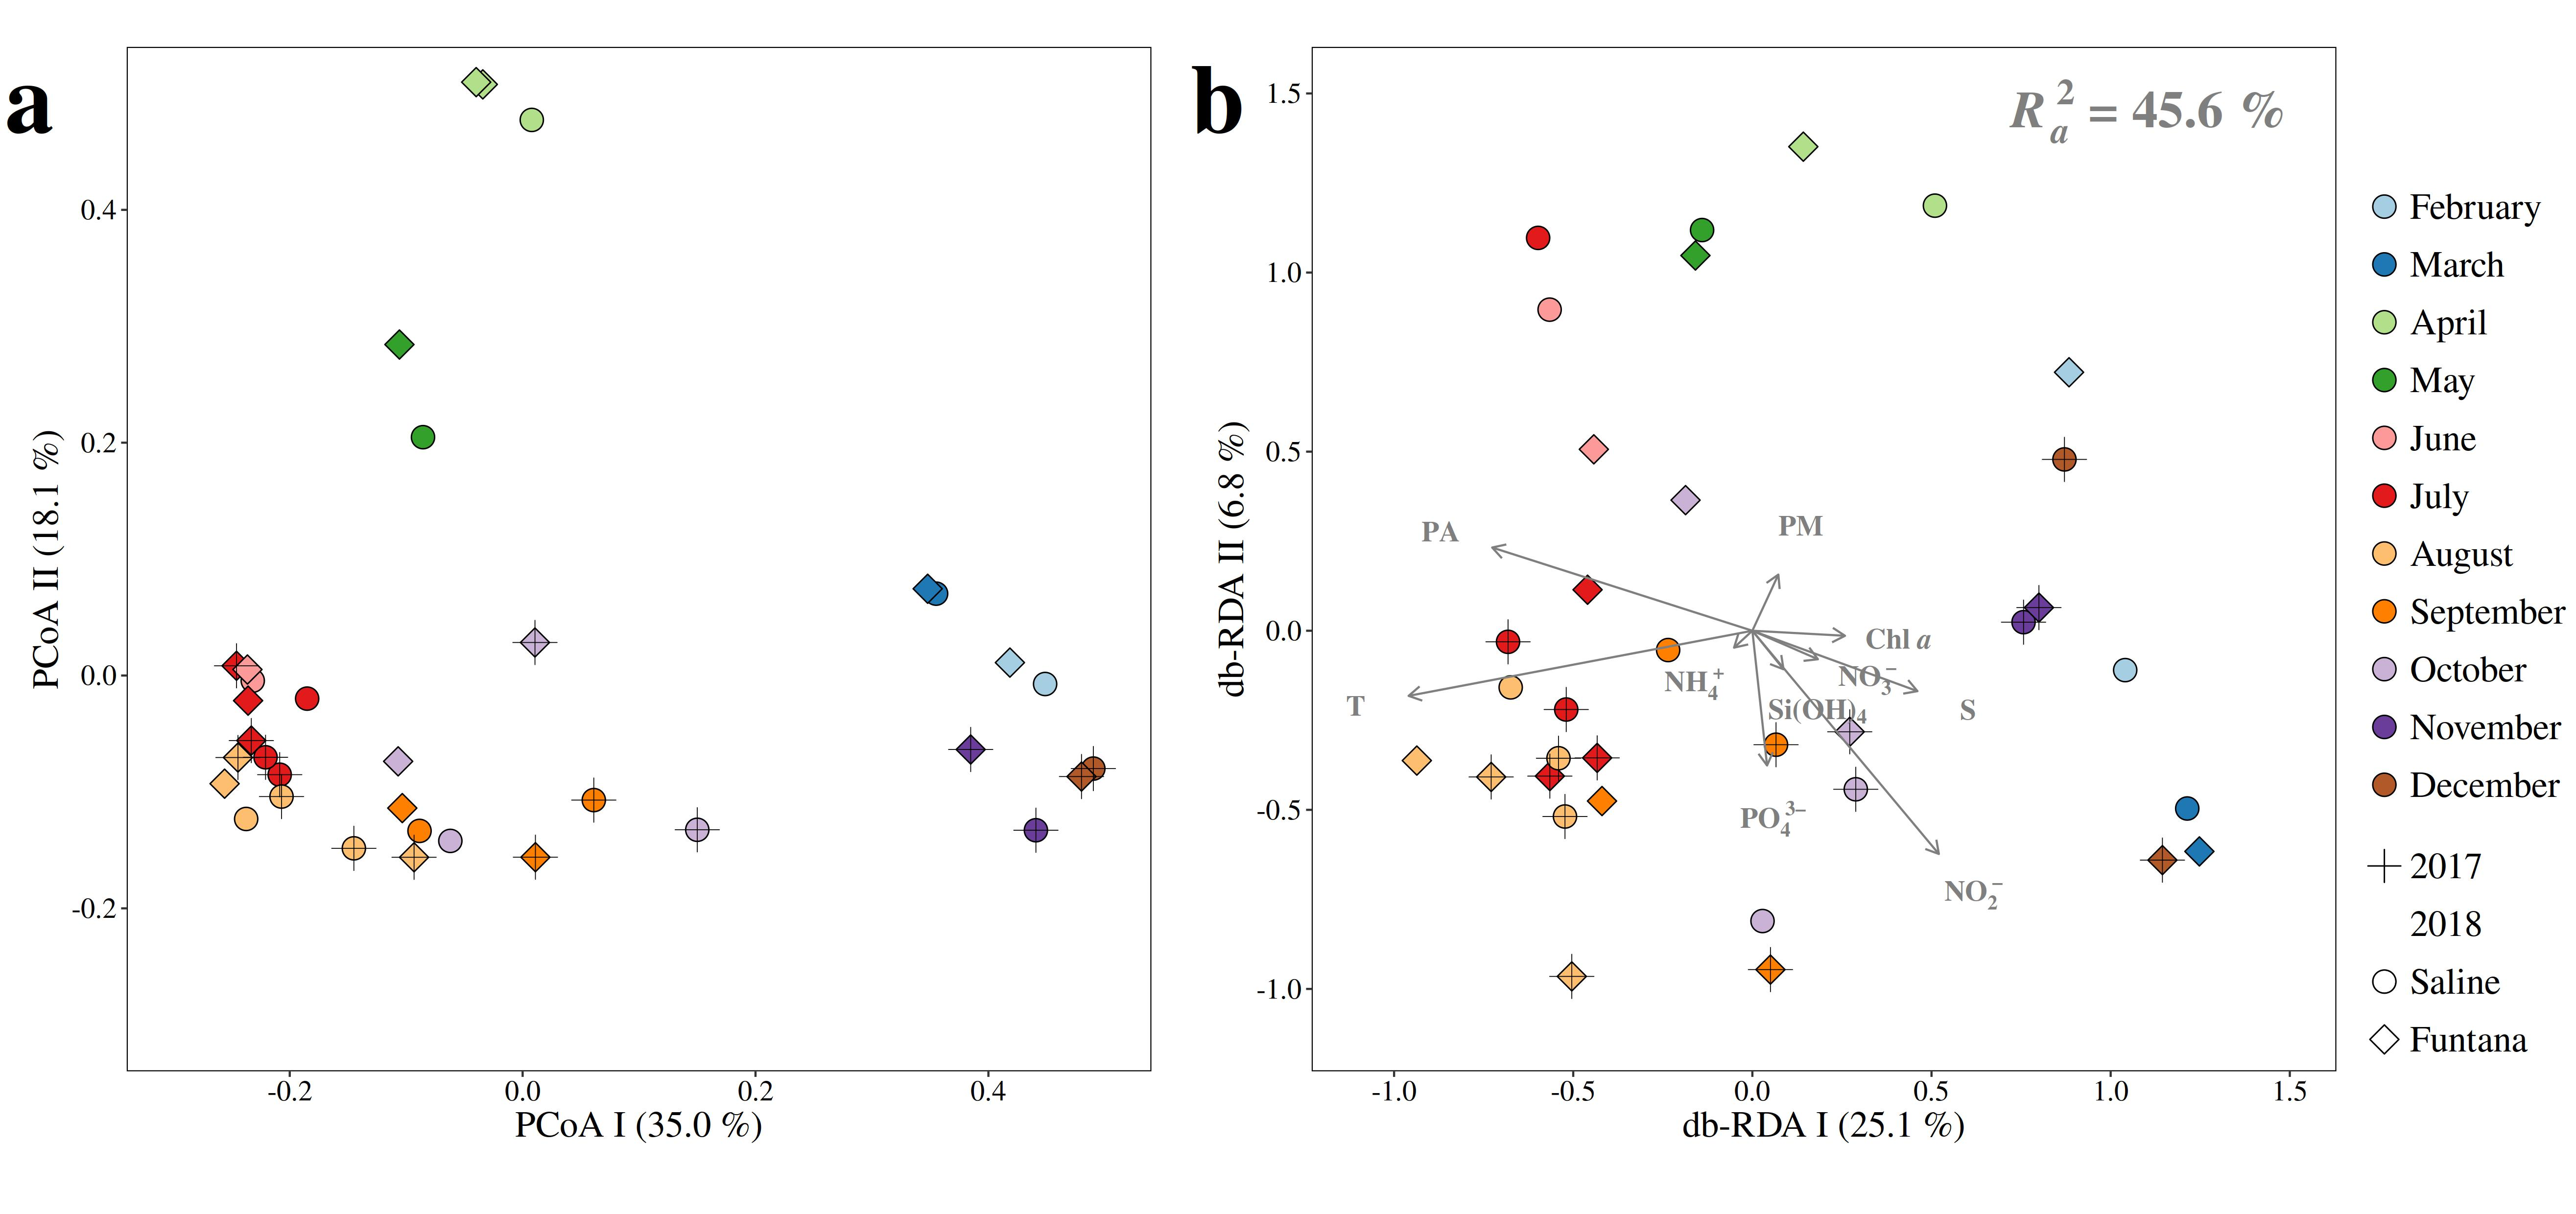
\includegraphics[width=0.9\linewidth]{../results/figures/pcoa_dbrda_figure} 

}

\caption{(a) Principal Coordinates Analysis (PCoA) of Bray-Curtis dissimilarities based on OTU abundances of bacterial and archaeal communities sampled in the Bay of Saline and Funtana. The proportion of explained variation by each axis is shown on the corresponding axis in parentheses. (b) Distance-based Redundancy Analysis (db-RDA) of Bray-Curtis dissimilarities based on the same community data sampled at the same locations and constrained by a set of environmental parameters (T -- temperature, S -- salinity, \ch{PO4^3-} -- orthophosphate, \ch{NH4^+} -- ammonium, \ch{NO2-} -- nitrite, \ch{NO3-} -- nitrate, \ch{Si(OH)4} -- silicic acid, PM -- particulate matter, Chl \textit{a} -- chlorophyll \textit{a}, and PA -- prokaryotic abundance). Scaling type 2 and fitted site scores were selected to construct the plot. The proportion of community data variation explained by environmental variables ($R^2_a$) is stated on the biplot, while the proportion of community data variation explained by each canonical axis is shown on the corresponding axis in parenthesis. Samples in both plots originating from different months, years, and stations are labeled in different shape and color.\label{pcoa_dbrda}}\label{fig:unnamed-chunk-1}
\end{figure}

\elandscape

\begin{figure}[H]

{\centering 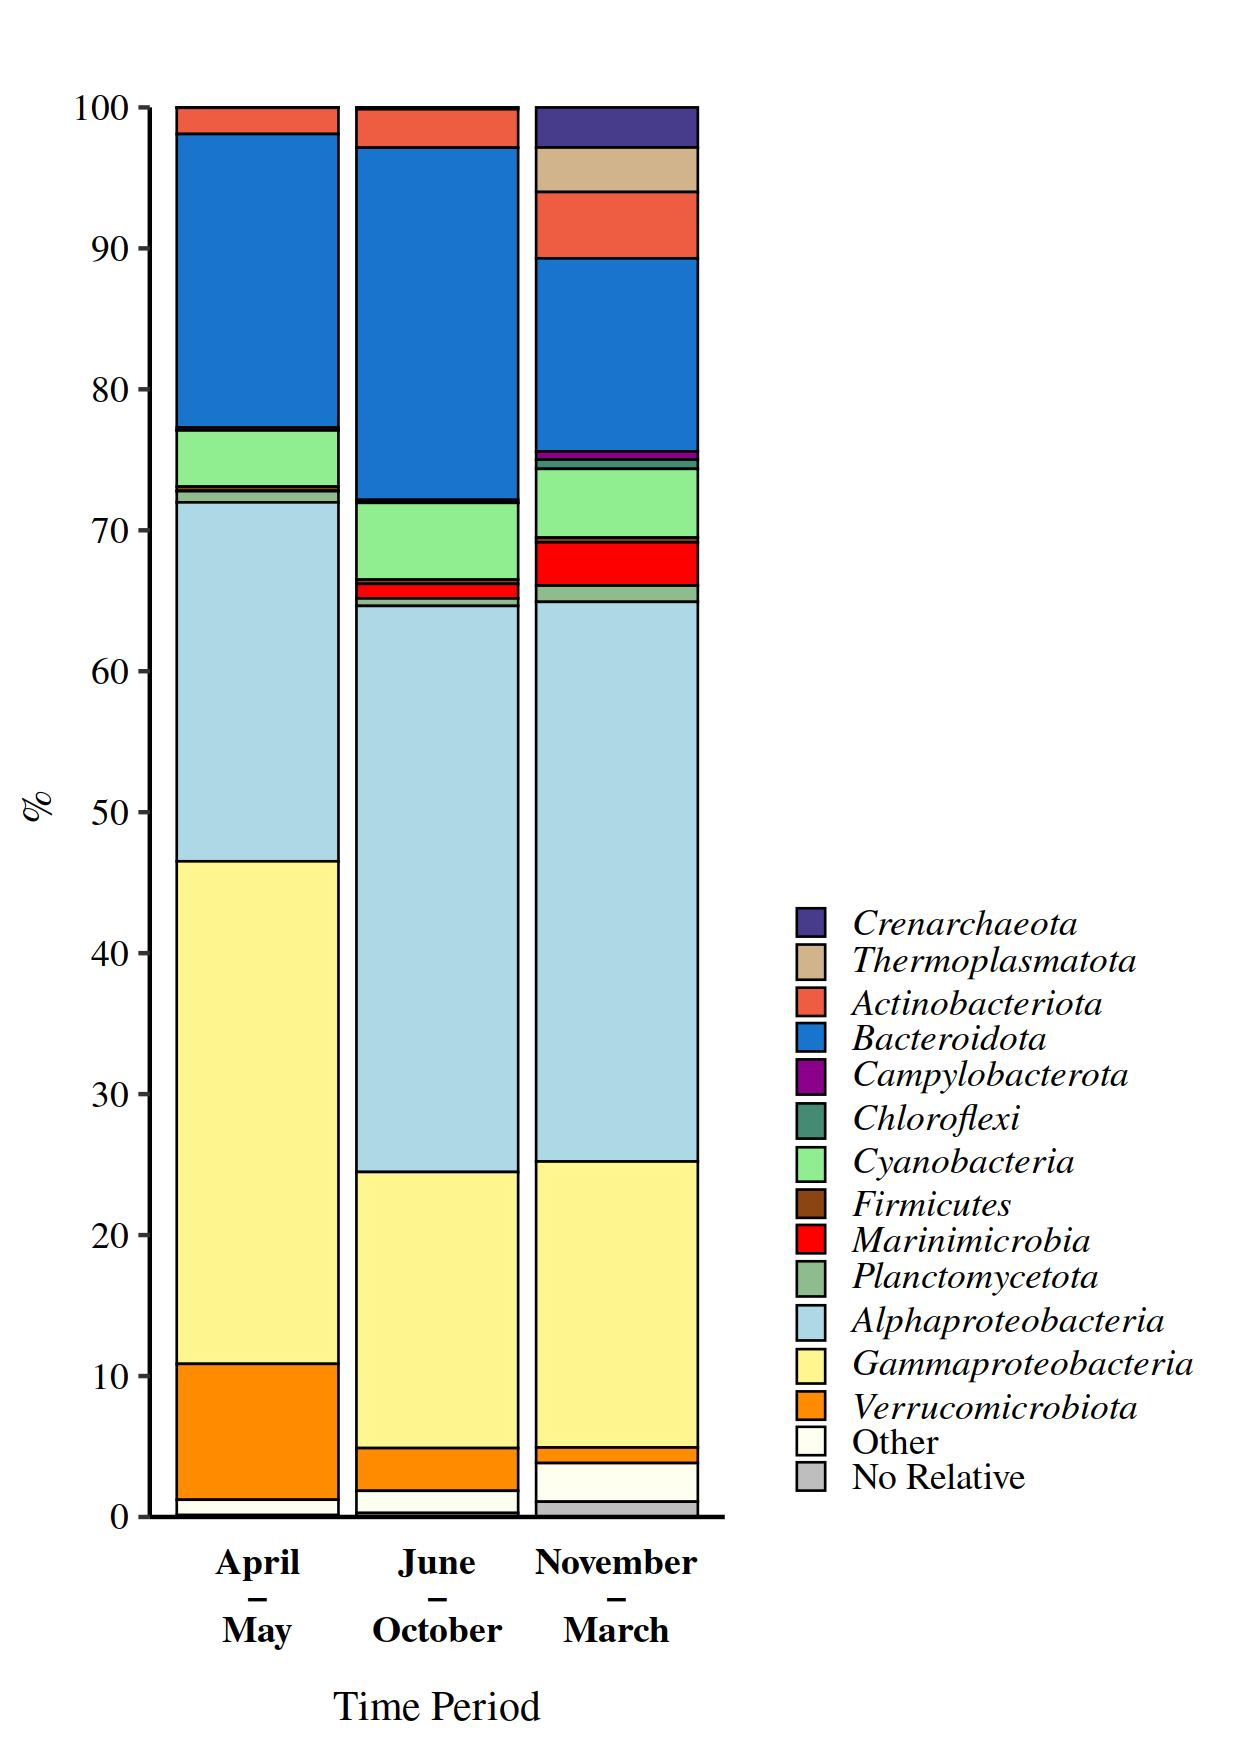
\includegraphics[width=1\linewidth]{../results/figures/community_bar_plot_month} 

}

\caption{Taxonomic classification and relative contribution of the most abundant ($\geq$ 1 \si{\percent}) bacterial and archaeal sequences during different time periods. No Relative -- sequences without known relatives\label{community_month}}\label{fig:unnamed-chunk-2}
\end{figure}

\begin{figure}[H]

{\centering 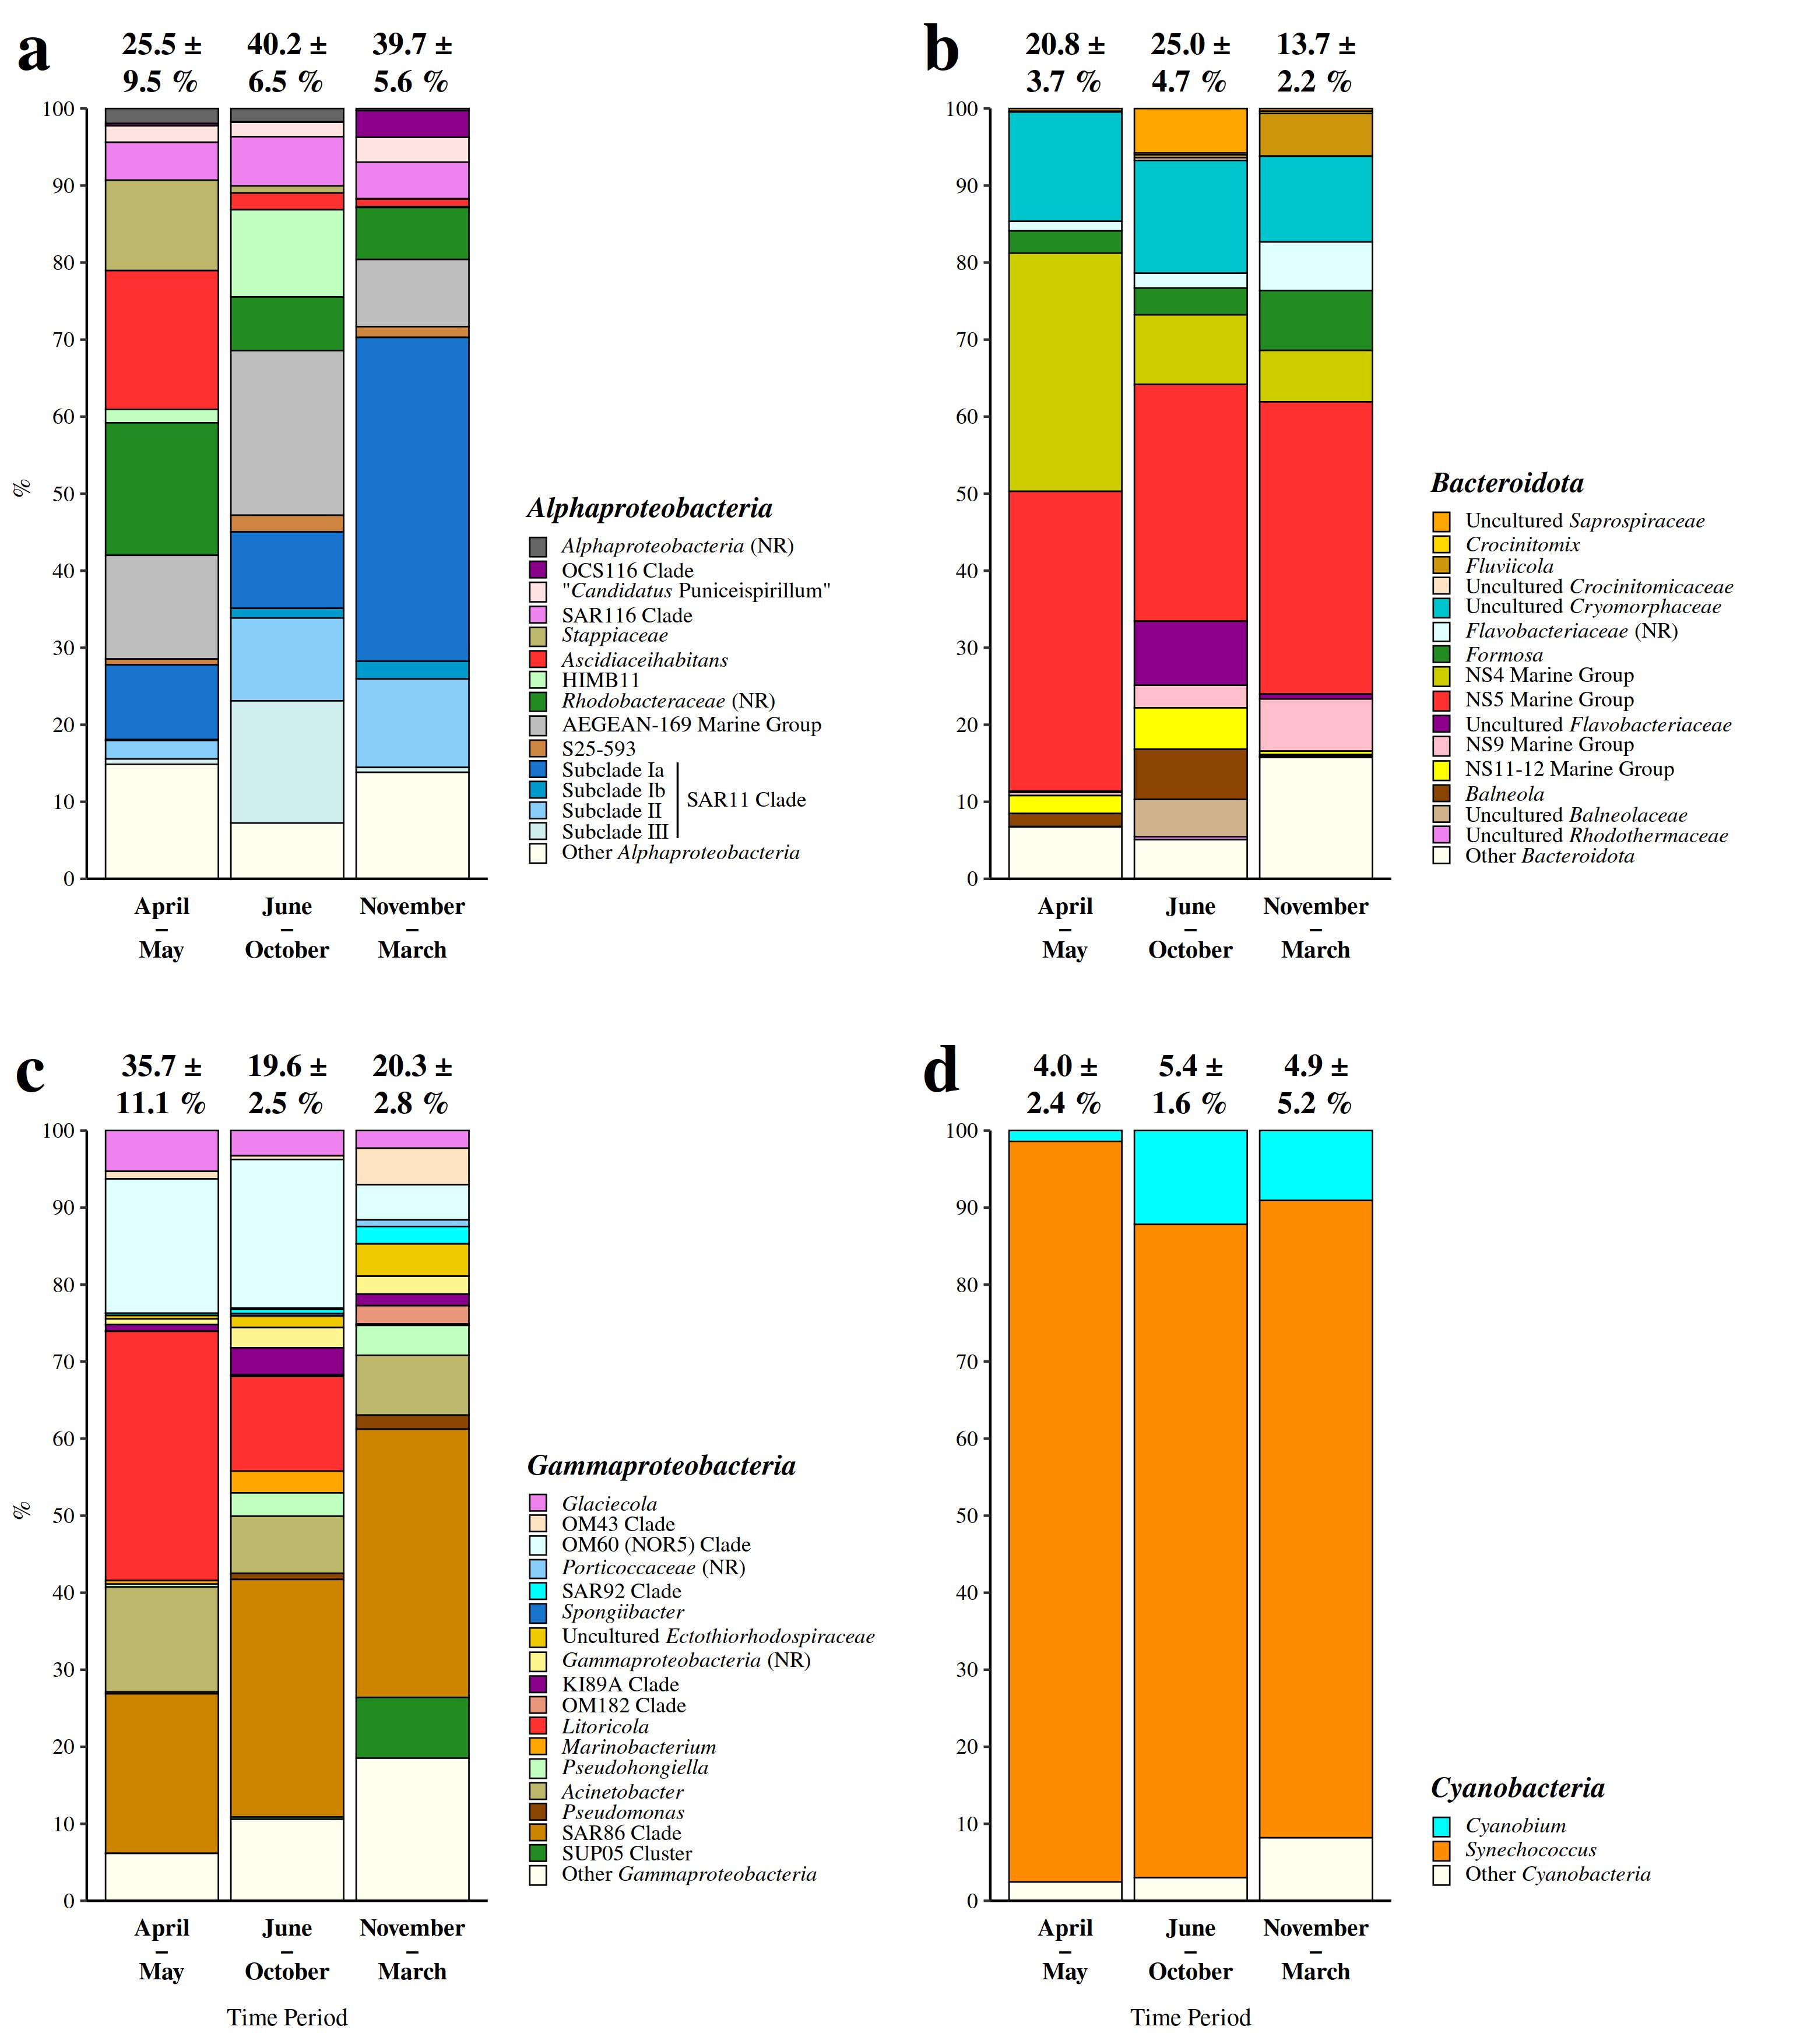
\includegraphics[width=1\linewidth]{../results/figures/community_bar_plot_month_taxa} 

}

\caption{Taxonomic classification and relative contribution of the most abundant sequences within \textit{Alphaproteobacteria} ($\geq$ 2 \si{\percent}) (a), \textit{Bacteroidota} ($\geq$ 1 \si{\percent}) (b), \textit{Gammaproteobacteria} ($\geq$ 1 \si{\percent}) (c), and \textit{Cyanobacteria} ($\geq$ 1 \si{\percent}) (d) during different time periods. The proportion of sequences classified into each of these taxa in the total bacterial and archaeal community is given above the corresponding bar. NR -- No Relative (sequences without known relatives within the corresponding group)\label{community_month_taxa}}\label{fig:unnamed-chunk-3}
\end{figure}

\end{document}
